\hypertarget{experiments}{
}

In the experimental stage of this research, two experiments are performed on two different datasets to analyze the overall quality of the synthetic image data generated by the various reflection models. The experiments conducted by Targhi for diffuse material classes are replicated and extended with synthesis using other reflection models, and the same setup is used on a new selection of material classes from the {\it PhoTex} database. The new selection of material classes have more glossy/shiny properties unlike the classes selected by Targhi, which should give a better indication for the quality of specularity simulated by Phong, Blinn-Phong and Torrance-Sparrow reflectance. 

\section{Preprocessing}\label{sec:preprocessing}
The {\it PhoTex} database consists of images recorded under a fixed point of view with varying light-source directions registered for each image. For the experiments, two datasets are chosen: a dataset according to the selection made by Targhi and another dataset with shiny properties to extend the experiments for the specular reflection models. 

After rendering new images for the materials and before extracting the features from the materials, the rendered images are set to zero-mean and unit-variance in order to make the features intensity-invariant. Since the diffuse and glossy/shiny materials have different image sizes, all images are cropped with respect to the center of the image to $200 \times 200$ pixels.

\subsection{Diffuse material classes}
Given that we are interested in reproducing some results from the experiments of Targhi, and measure performance of more complex reflection models with respect to the Lambertian reflection model he applied for synthesis, we need to select the same material classes he used in his experiment. The material classes are shown in figure \ref{fig:PhoTexData}. These classes represent materials such as plaster and paper, but also repeating primitives such as pebbles and peas.

From each material class, 40 images with certain slant and tilt angles are selected. The selected slant angles are $\{30^0, 45^0,60^0,75^0\}$. The images under a slant of $30^0$ have four different tilts, $\{0^0, 90^0, 180^0, 270^0\}$. The images with slants $\{45^0,60^0,75^0\}$ have tilts of $\{0^0,30^0,60^0,..., 300^0,330^0\}$. 

%\begin{comment}
\begin{figure}[h]
	\begin{center}
		\subfigure[aaa]{
\epsfig{file=images/db/aaa.eps, width=0.15\linewidth}}
		\subfigure[aab]{
\epsfig{file=images/db/aab.eps, width=0.15\linewidth}}
		\subfigure[aaj]{
\epsfig{file=images/db/aaj.eps, width=0.15\linewidth}}
		\subfigure[aam]{
\epsfig{file=images/db/aam.eps, width=0.15\linewidth}}
		\subfigure[aan]{
\epsfig{file=images/db/aan.eps, width=0.15\linewidth}}

		\subfigure[aao]{
\epsfig{file=images/db/aao.eps, width=0.15\linewidth}}
		\subfigure[aar]{
\epsfig{file=images/db/aar.eps, width=0.15\linewidth}}
		\subfigure[aas]{
\epsfig{file=images/db/aas.eps, width=0.15\linewidth}}
		\subfigure[aba]{
\epsfig{file=images/db/aba.eps, width=0.15\linewidth}}
		\subfigure[abj]{
\epsfig{file=images/db/abj.eps, width=0.15\linewidth}}

		\subfigure[abk]{
\epsfig{file=images/db/abk.eps, width=0.15\linewidth}}
		\subfigure[acc]{
\epsfig{file=images/db/acc.eps, width=0.15\linewidth}}
		\subfigure[acd]{
\epsfig{file=images/db/acd.eps, width=0.15\linewidth}}
		\subfigure[ace]{
\epsfig{file=images/db/ace.eps, width=0.15\linewidth}}
		\subfigure[adb]{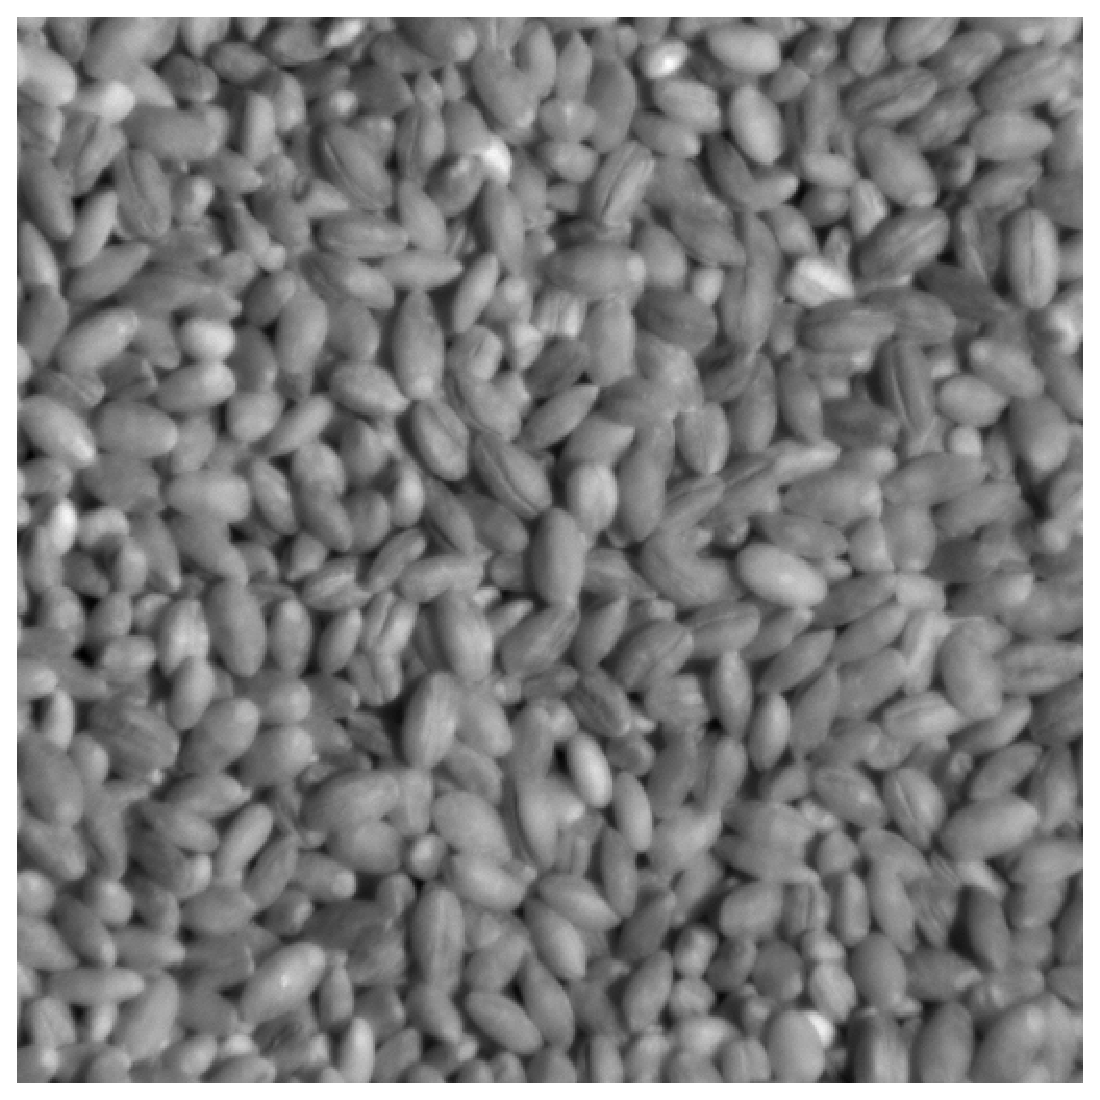
\epsfig{file=images/db/adb.eps, width=0.15\linewidth}}

		\subfigure[adc]{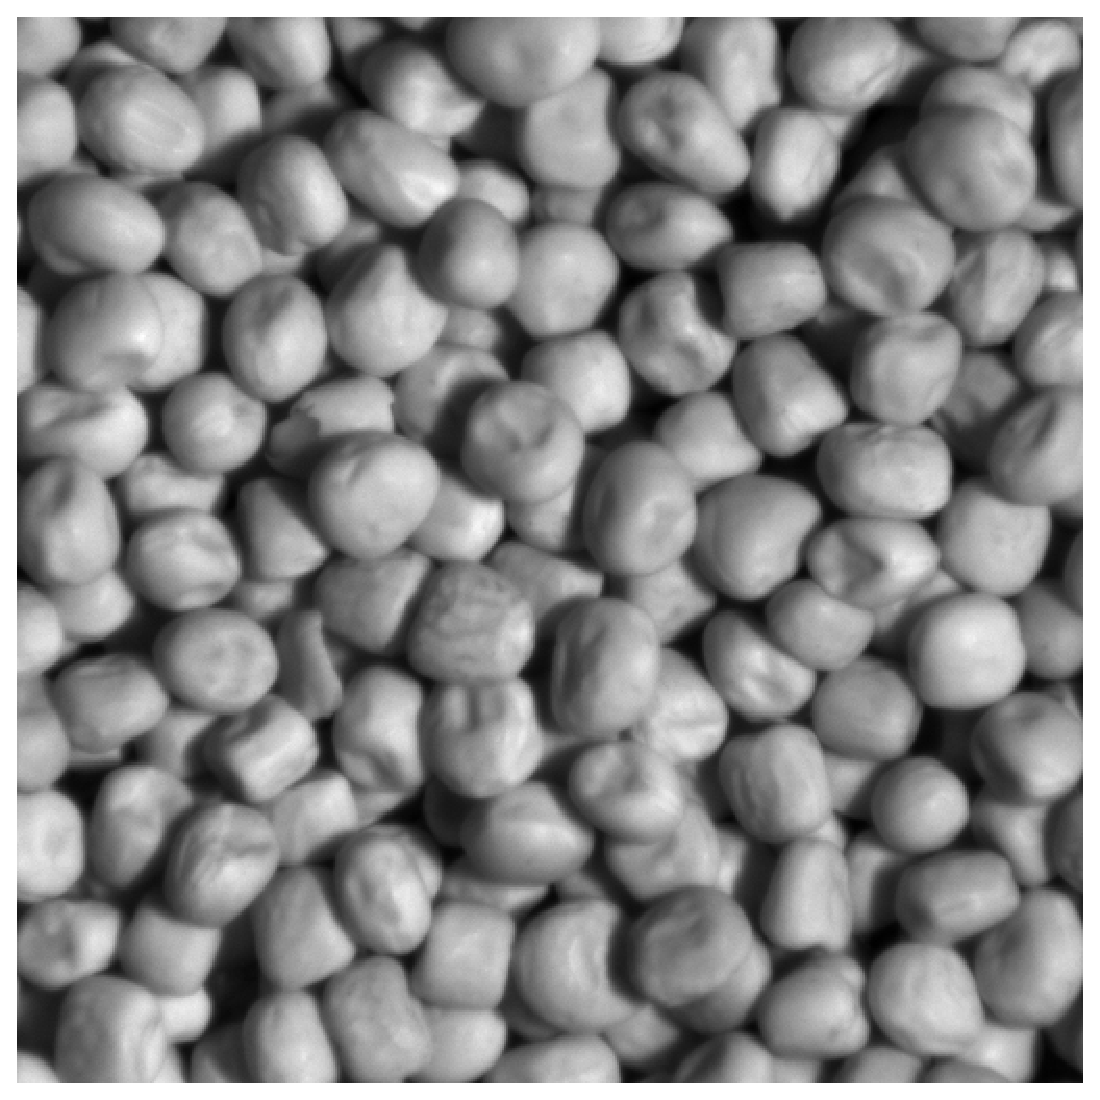
\epsfig{file=images/db/adc.eps, width=0.15\linewidth}}
		\subfigure[add]{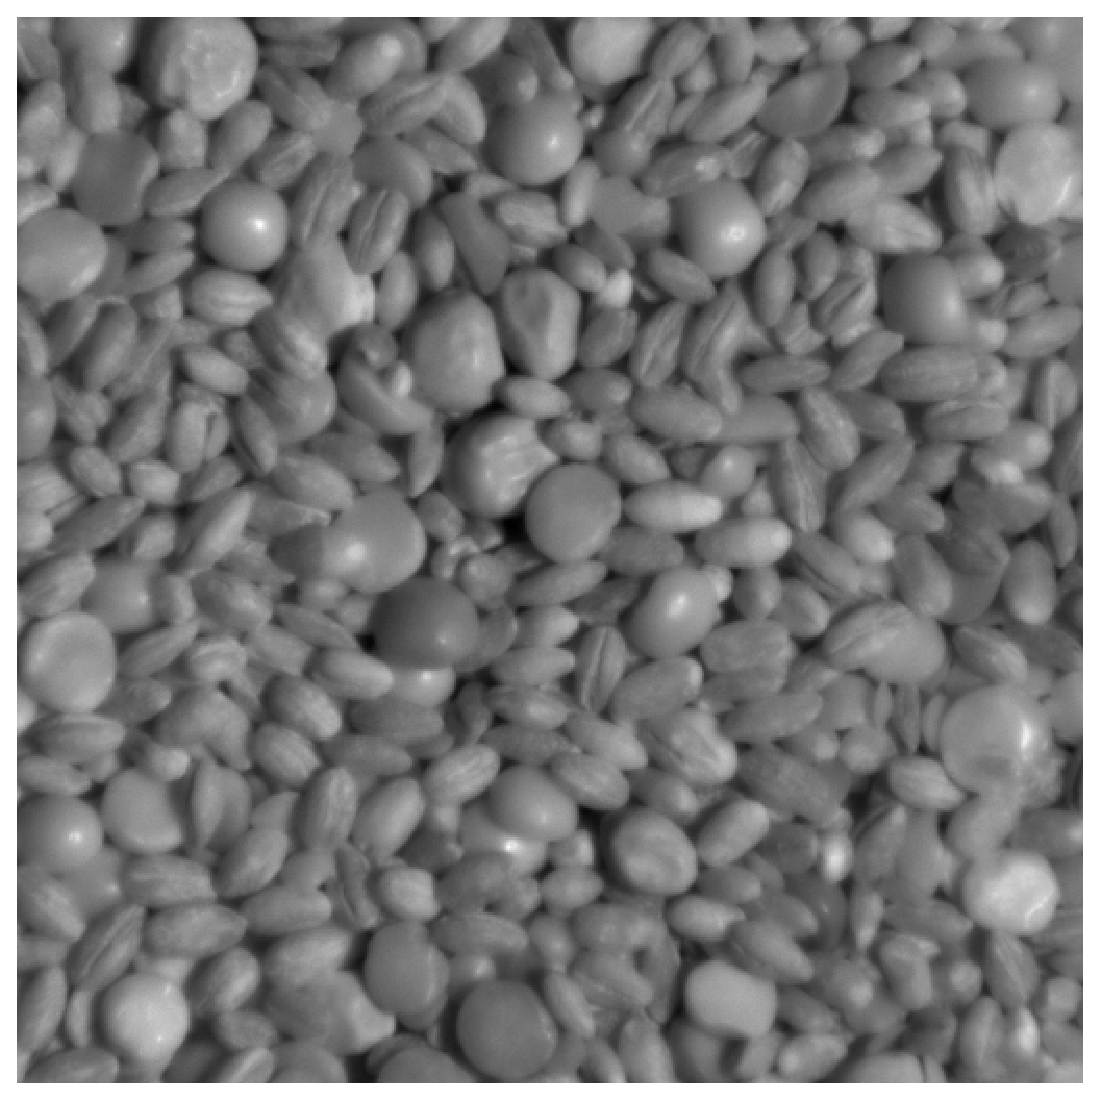
\epsfig{file=images/db/add.eps, width=0.15\linewidth}}
		\subfigure[ade]{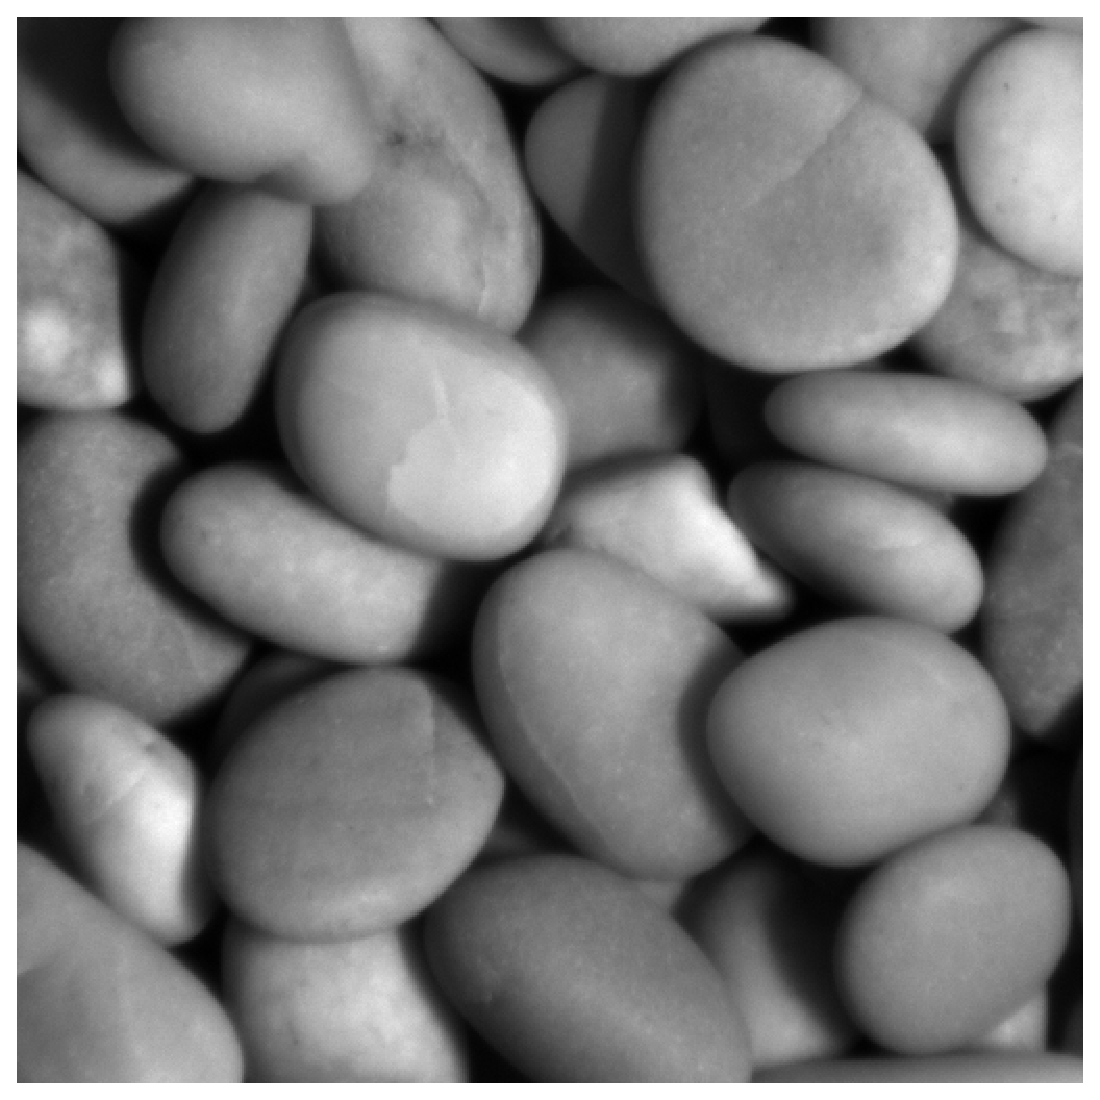
\epsfig{file=images/db/ade.eps, width=0.15\linewidth}}
		\subfigure[adg]{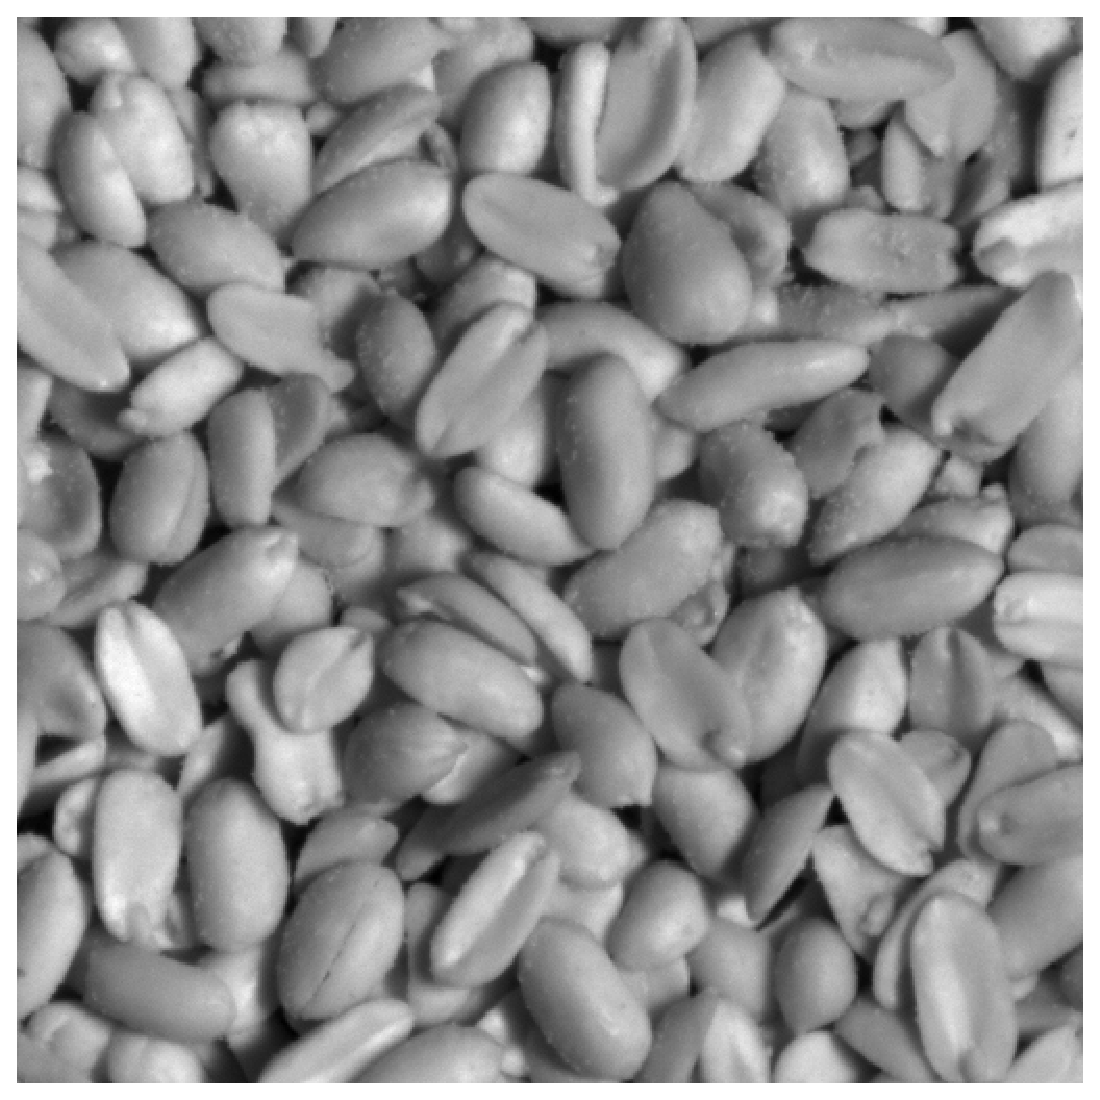
\epsfig{file=images/db/adg.eps, width=0.15\linewidth}}
		\subfigure[adh]{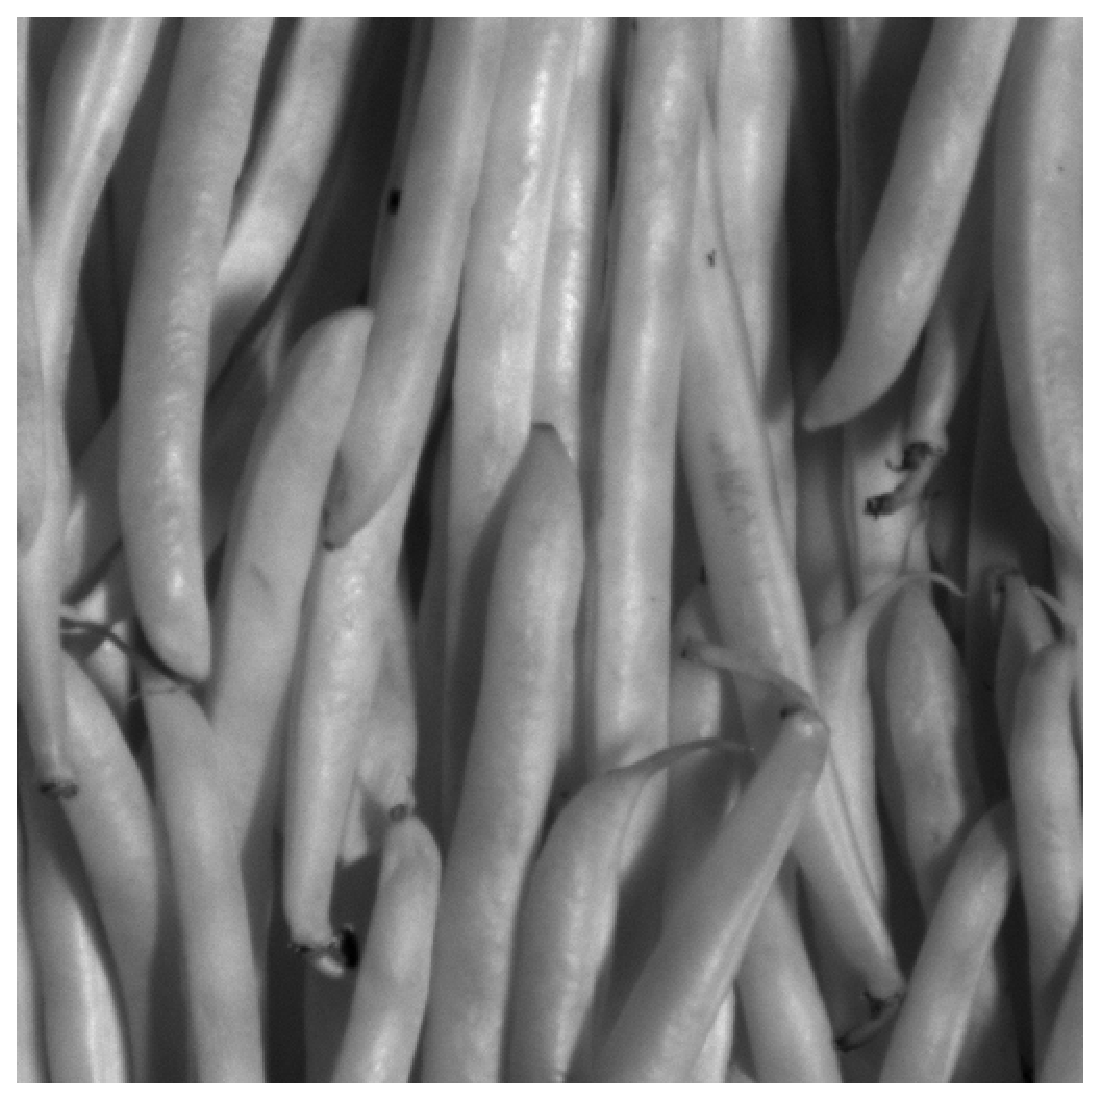
\epsfig{file=images/db/adh.eps, width=0.15\linewidth}}
	\end{center}
	\caption{{\it Classes taken from the PhoTex database for the diffuse material dataset. The example images are registered under a slant of $30^0$ and a tilt of $0^0$.}}
	\label{fig:PhoTexData}
\end{figure}
%\end{comment}

\subsection{Shiny material classes}
Because three out of five reflection models simulate specularity only, the previous dataset might not be good enough to measure improvements made by these reflection models. For this reason, a new dataset is selected from the {\it PhoTex} database with more specular properties. 

The material classes selected are shown in figure \ref{fig:PhoTexData2}. This dataset consists of 10 material classes, recorded under a slant of $75^0$ and tilts of $0^0$ to $350^0$ in increments of $10^0$, giving a total of 36 images for each material class. The material classes are shown in figure \ref{fig:PhoTexData2}, and represent different machined surfaces of nickel. We can only select 36 images instead of 40 because these materials are only recorded under a slant of $75^0$ in the {\it PhoTex} database and we would like to be able to select configurations of 4 images with tilts incrementing in steps of $90^0$. The reason for this will be explained in section \ref{sec:Experiments}.

%\begin{comment}
\begin{figure}[h]
	\begin{center}
		\subfigure[g2]{
\epsfig{file=images/db/g2.eps, width=0.15\linewidth}}
		\subfigure[g4]{
\epsfig{file=images/db/g4.eps, width=0.15\linewidth}}
		\subfigure[g8]{
\epsfig{file=images/db/g8.eps, width=0.15\linewidth}}
		\subfigure[g16]{
\epsfig{file=images/db/g16.eps, width=0.15\linewidth}}
		\subfigure[r8]{
\epsfig{file=images/db/r8.eps, width=0.15\linewidth}}

		\subfigure[t16]{
\epsfig{file=images/db/t16.eps, width=0.15\linewidth}}
		\subfigure[t63]{
\epsfig{file=images/db/t63.eps, width=0.15\linewidth}}
		\subfigure[vm16]{
\epsfig{file=images/db/vm16.eps, width=0.15\linewidth}}
		\subfigure[vm32]{
\epsfig{file=images/db/vm32.eps, width=0.15\linewidth}}
		\subfigure[vm63]{
\epsfig{file=images/db/vm63.eps, width=0.15\linewidth}}
	\end{center}
	\caption{{\it Classes taken from the PhoTex database for the glossy/shiny material dataset. The example images are registered under a slant of $75^0$ and a tilt of $20^0$.}}
	\label{fig:PhoTexData2}
\end{figure}
%\end{comment}

\section{Reflection model parameters}\label{sec:ParameterSetting}
The reflection models used in the process of synthesis need material dependent parameters to be set such as the parameter for the specular lobe size or surface roughness. However, these parameters are not available for the materials present in the database in the case of the micro-facet models, and in the case of the empirical models there are no known 'good' values for the parameters to be set. To set these values, the parameters are computed using a gradient descent procedure with a total sum of squares error estimation:

		\begin{eqnarray*}
			Err(A,A') = \sum_{i=1}^n (a_i - a_i')^2
		\end{eqnarray*}
 
Where $A$ is the original image from the {\it PhoTex} database, and $A'$ is the synthesized image that mimics the original image. By calculating the squared per-pixel error from the original image and the synthetic image, and accumulate this error over all pixels we find the error of the synthetic image with respect to the original image. Accumulating this error over a set of synthetic images with its respective set of original images will give an estimation of the total error for a given parameter configuration. By accumulating the error over sets of images instead of using just one image for the parameter estimation, we hope to avoid potential local minima in the gradient descend. Both synthetic and original image are preprocessed to have zero-mean and unit-variance before the error is calculated, since the features will be extracted from such preprocessed images.

Because the number of materials and the number of parameters to be estimated for each reflection model turn out to be large in total and the error for gradient descend needs to be computed over sets of images, a simplified gradient descend is done. Each parameter is estimated using a defined range of possible values. For the microfacet models, the roughness of a material is $m \in \{0.1, 0.3, 0.5, 0.7, 0.9\}$. The Fresnel coefficient is $R_f \in \{0.01, 0.03, 0.05, 0.07, 0.09\}$ for the diffuse material set and $R_f \in \{0.1, 0.3, 0.5, 0.7, 0.9\}$ for the shiny/glossy material dataset. The shininess constant $\alpha$ for Phong and Blinn-Phong reflection corresponds to a value in $\{0.001, 0.01, 1.0, 5.0 10.0, 40.0\}$ and the specular reflection coefficient $k_s$ corresponds to a value in $\{0.001 0.01 0.1 0.25 0.5 0.75 1.0\}$. 

The surface albedo and surface normals needed for this procedure are derived for each material from images with light directions registered with a slant of $30^0$ and tilts of $\{0^0, 90^0, 180^0, 270^0\}$. The choice for this configuration of angles over the hemisphere is based on the quality of the recovered surface albedo since a non-uniform configuration of tilts gives rise to specularity in the surface albedo. With a uniform choice of angles over the hemisphere, these outliers have minimal influence. Both RANSAC and surface normal smoothing are discarded from the experiments since applying these methods showed significant bigger accumulated errors in the recovery of the surface albedo and surface normals with respect to the accumulated error of the uniform configuration.

\section{Experimental Setup}\label{sec:Experiments}
In this section, two experiments are described that will be applied on both the diffuse and glossy/shiny material dataset. Three different training sets are considered. These training sets are meant to be used for photometric stereo to compute the surface albedo and surface normals. Listed are the training sets for this procedure and are taken from each class separately:

\begin{itemize}
	\item{\textit{T1} - 20 images {\it pseudo-randomly} selected, as proposed by Targhi}
	\item{\textit{T3} - 4 images randomly selected from \textit{T1}, as proposed by Targhi}
	\item{\textit{TT} - the 4 images under a slant of $30^0$ used for finding parameters, as described in section \ref{sec:ParameterSetting}}
\end{itemize}

Similar results to that of Targhi's experiments have been replicated, but exact results are hard to obtain since the quality of the synthetic image data depends strongly on the input images for the photometric stereo. Targhi uses a {\it pseudo-random} selection procedure to obtain the $T1$ set, where pseudo-random is defined as selecting slant and tilt angles to be uniform over the hemisphere. Unfortunately this pseudo-random selection procedure is not explained in further detail, making it hard to obtain the similar training sets.

Pseudo-random in this research is defined as follows: for every slant, a number of tilts is available. There are three configurations of tilts possible such that the hemisphere is covered uniformly when using tilts in increments of $90^0$. To select the 20 images for each class, 5 slants are chosen randomly, and for each slant a configuration of 4 tilts is chosen randomly. Note that in the case of a slant of $30^0$, there is only 1 configuration possible. 

\subsection{Experiment A}
In this experiment, we mimic the images from the $T1$ training set to obtain a synthetic training set. This means that for each training set ($T1$, $T3$ and $TT$) we recover the surface albedo and surface normals. With the recovered maps we create synthetic datasets using the slant and tilt angles from the $T1$ dataset for each of the reflection models, creating a total of 20 synthetic images per material class. The training of the material models will be done using these synthetic datasets, and the test images --- images that are not in $T1$ --- are selected from the original {\it PhoTex} dataset.

\subsection{Experiment B}
To further investigate the quality of the synthetic image data, an experiment similar to experiment A is conducted, but now instead of mimicking only the images in the $T1$ training set, we mimic all images from the original datasets. We then perform random sub-sampling validation by measuring classification performance of the models derived from synthetic image data and tested against the original dataset. Synthetic training sets are randomly selected from the synthetic data and a test set is randomly selected from the original data. This process of random sub-sampling validation is repeated a 1000 times to average the results. The training set will be increased in the number of images used for constructing the material models until all synthetic images are used for training. 

The idea behind this experiment is as follows: when one would do this experiment using the original {\it PhoTex} image data, perfect classification accuracy is achieved when all images are used for training material models, and 20 images are used for testing. Clearly this is a case overfitting. However, if we would achieve perfect classification accuracy using only synthetic image data, we have found a model that perfectly mimics the original data. 

\section{Results}\label{sec:Results}
In this section, the results for both experiment A and B are reported on the diffuse and glossy/shiny material database. We employ the configuration of Broadhurst for the construction of the marginal histograms by having 25 bins. The number of eigencomponents differs, since we measured maximum performance with 13 eigencomponents.

\subsection{Diffuse material dataset}
Table \ref{tab:DiffuseResultsA} shows the results for experiment A. The results are averaged over 5 repetitions of the experiment. As it can be seen, the original image data performs really well when training on one half of the dataset and testing on the other half with an average accuracy of \%95.1525. The accuracy for the synthetic data degrades by around 13\% - 16\% for the different training sets. There is a clear gap between the quality of the synthetic image data and the original image data that has not been covered by any of the reflection models. When comparing the reflection models we have to conclude that no significant improvements are made, not even when comparing the more sophisticated reflection models with the Lambertian reflection model. 
 
\begin{table}
	\center
	\begin{tabular}{l|c|c|c|r}
	Method 				&	T1  	&	T3 		&	TT	\\
	\hline
	Original			&	95.1525	&	95.1525 &	95.1525	\\
	Lambertian 			&	81.2212	&	79.7950	&	78.8125	\\
	Phong 				&	81.2440	&	76.7650 &	79.0825	\\
	Blinn-Phong 		& 	82.3030 &	79.9825 &	78.7163	\\
	Torrance-Sparrow 	&	81.9465 &	79.8075 &	81.0487	\\
	Oren-Nayar 			&	82.1475 &	79.8888 &	79.8187	\\
	\end{tabular}
	\caption{{\it Mean accuracy over 5 repetitions for the diffuse material dataset for 20 images in the training set and 20 images in the test set}}
	\label{tab:DiffuseResultsA}
\end{table}

In figure \ref{fig:DiffusePlotB}, we plot the accuracy as a function of the increasing number of images used for material model construction until all images from the original dataset are used. As with experiment A, experiment B has been repeated 5 times to average results. 

The plots suggest that again little to no improvement is made when comparing reflection models in the case of the $T3$ and $TT$ training sets. The fact no improvements are measured can be explained by how the photometric stereo does not recover the surface albedo and surface normals very well from the $T3$ and the $TT$ datasets. However, for the $T1$ training set we observe that an improvement of ~3\% is measured on top of the Lambertian reflectance for some of the reflectance models. 

Table \ref{tab:DiffuseResultsB} shows the mean and standard deviation for 40 images in the training set and 20 randomly selected images in the test set when using the $T1$ training set for photometric stereo. In the first row, we show performance of the original data to construct the material models and report an almost perfect classification accuracy. This is to be expected since we are overfitting. When using only synthetic image data however, the accuracy drops about 11\% - 14\%. When comparing the reflection models, some improvements with respect to Lambertian reflectance are reported. 

The best performing model is Blinn-Phong with an accuracy of 88.4347\%, followed up by Torrance-Sparrow with 87.8393\% accuracy , both performing better than Phong reflectance. Oren-Nayar for diffuse reflectance also performs better than Lambertian reflectance. The results of the three better performing reflection models have been positively tested on significance level of 5\% using a paired T-test. The results in the table and plots suggest that a more physically based approach can increase the quality of the synthetic images, since the purely empirical based Phong reflectance performs similar or worse than Lambertian reflectance in all experiments. It also suggests that using more images for photometric stereo improves the quality of the surface albedo and surface normals recovery, provided that the light sources are distributed uniformly over the hemisphere.

\begin{figure}[H]
	\begin{center}
		\subfigure[T1 dataset]{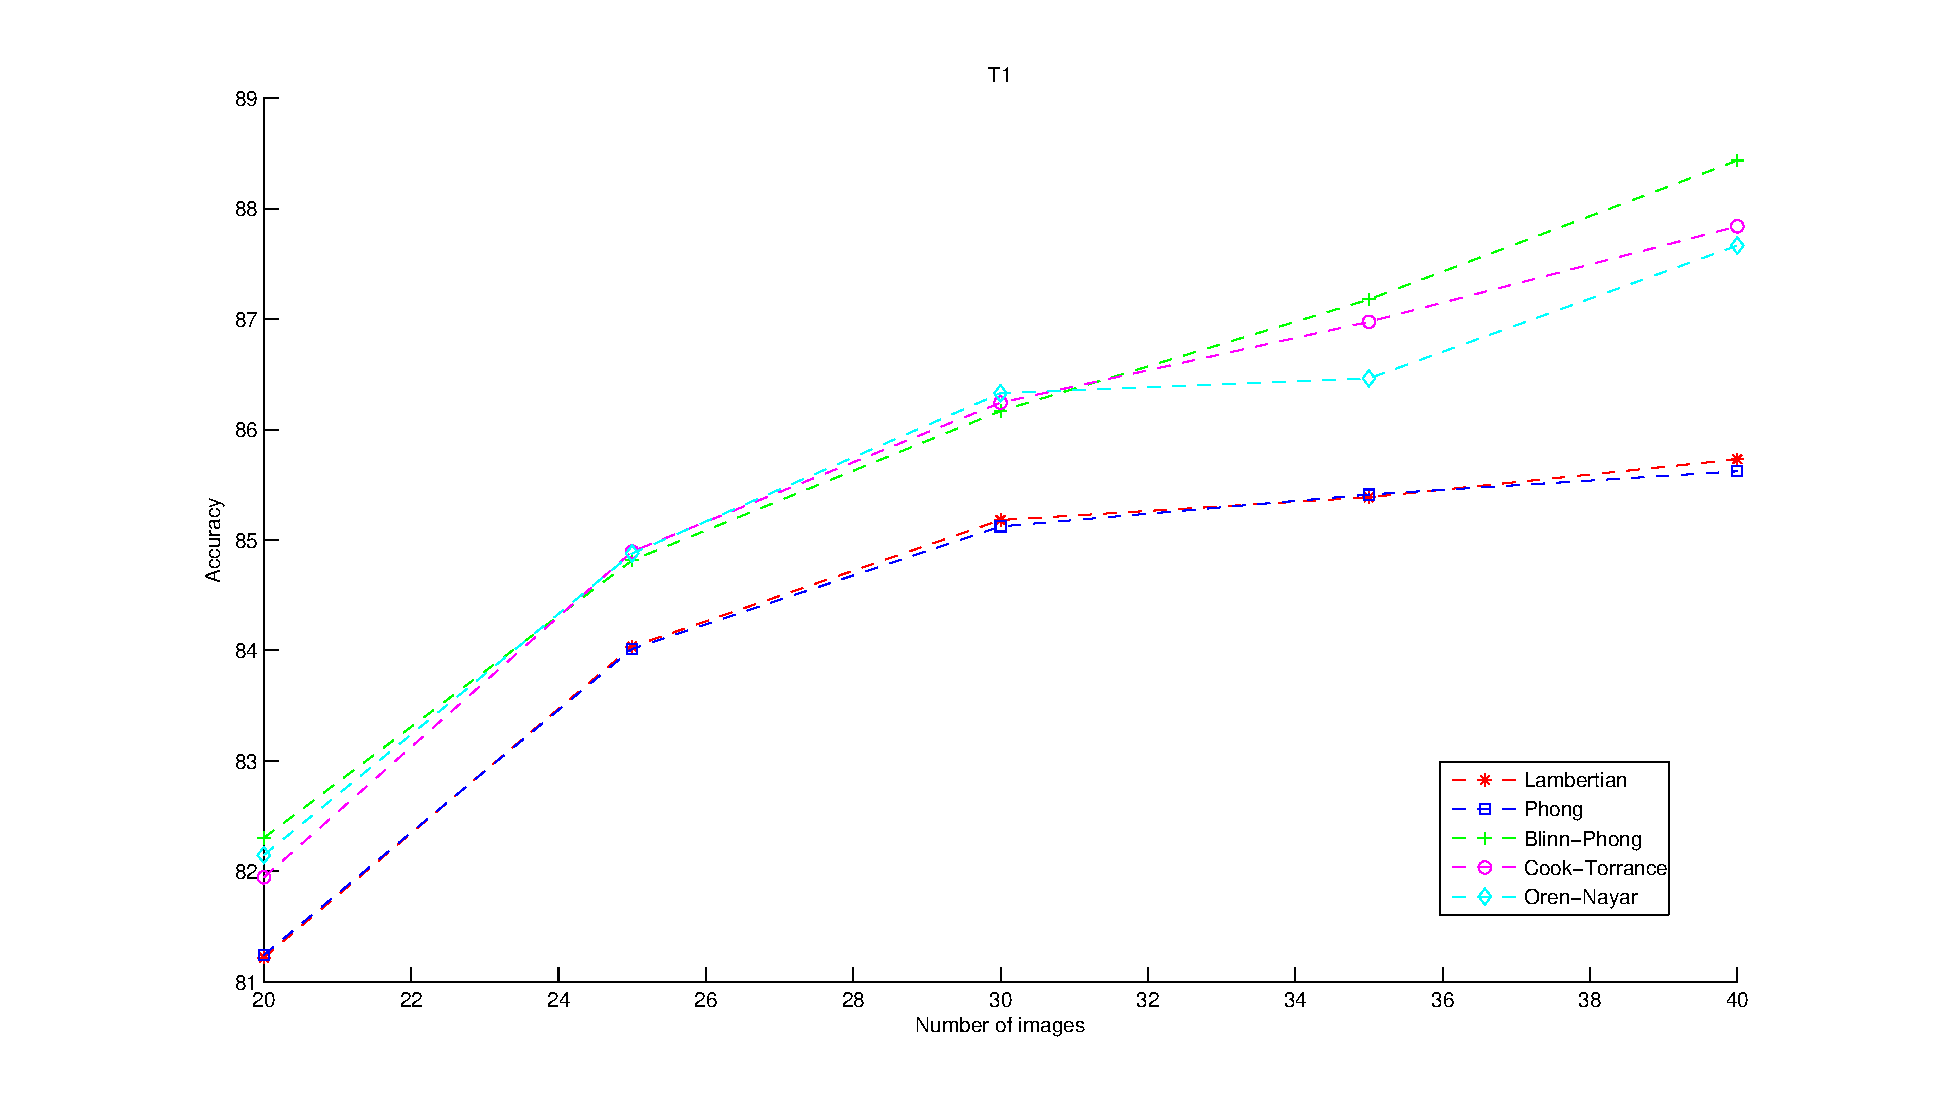
\epsfig{file=images/results/T1.eps, width=0.75\linewidth}}
		\subfigure[T3 dataset]{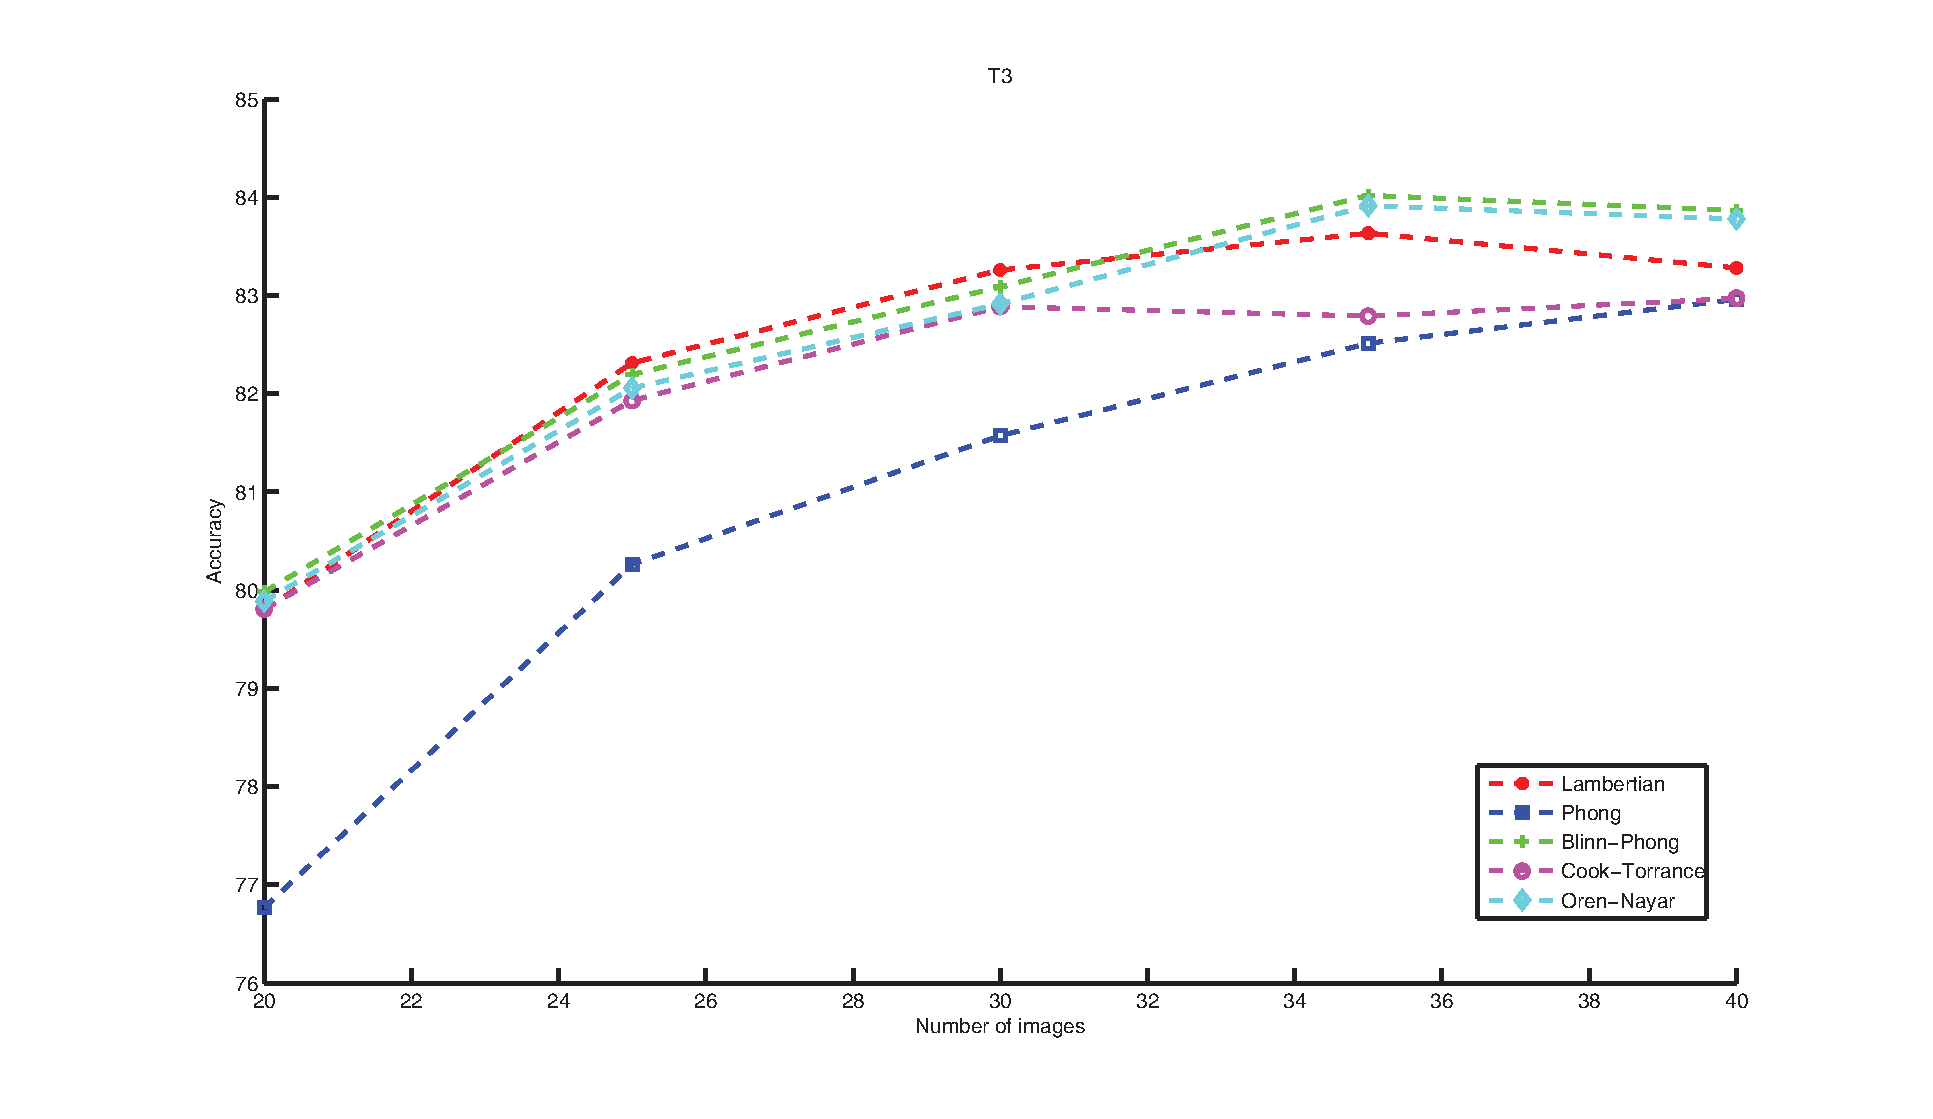
\epsfig{file=images/results/T3.eps, width=0.75\linewidth}}
		\subfigure[TT dataset]{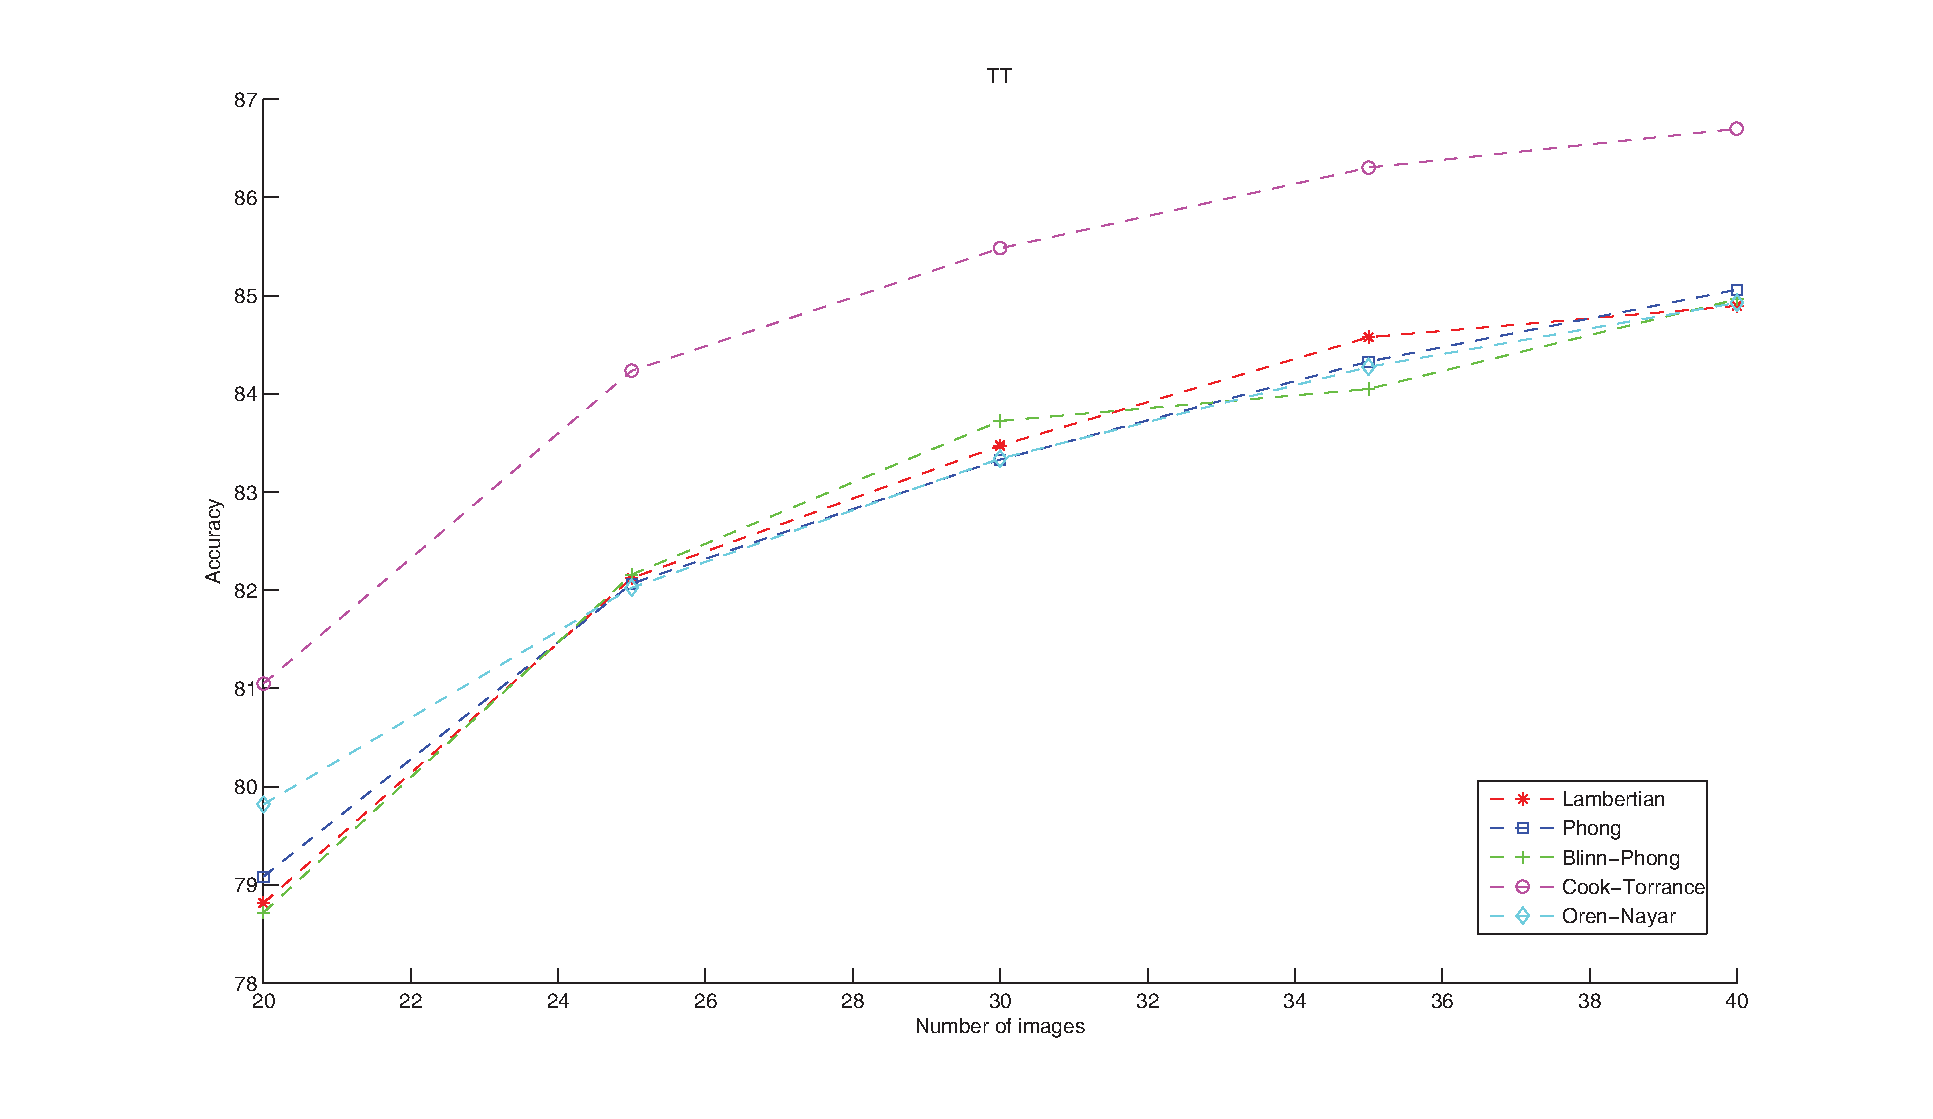
\epsfig{file=images/results/TT.eps, width=0.75\linewidth}}
	\end{center}
	\caption{{\it Results on the T1, T3 and TT dataset for diffuse materials.}}
	\label{fig:DiffusePlotB}
\end{figure}

\begin{table}
	\center
	\begin{tabular}{l|c|r}
	Method 				&	T1 - mean 	& T1 - std \\
	\hline
	Original			&	99.4912		& 0.232 \\
	Lambertian 			&	85.3313		& 2.386 \\
	Phong 				&	85.6222		& 2.451 \\
	Blinn-Phong 		& 	88.4347 	& 1.839 \\
	Torrance-Sparrow 	&	87.8393 	& 2.036 \\
	Oren-Nayar 			&	87.6650 	& 2.322 \\
	\end{tabular}
	\caption{{\it Mean accuracy and standard deviation over 5 repetitions for the diffuse material dataset for 40 images in the training set and 20 images in the test set}}
	\label{tab:DiffuseResultsB}
\end{table}

\subsection{Shiny/glossy material dataset}
For the experiments on the shiny/glossy material dataset we dropped the Phong reflectance for further investigation because of the results found on the diffuse material dataset. We also do not report on results on the $T3$ and $TT$ training sets since these datasets resulted in no significant results in experiment B on the diffuse dataset.

In table \ref{tab:SpecularResultsA} we report the accuracy of the different reflectance models where we have 20 images in the training set and the remaining images in the test set. We observe that the accuracy using synthetic image data has decreased drastically compared to the diffuse material dataset. The difference in accuracy is around 38\% between the original data and the synthetic data. We expect that these results are caused by the poor recovery of the surface albedo and surface normals, since our photometric stereo approach uses a Lambertian surface assumption and the materials in this dataset have a shiny/glossy nature. 

\begin{table}
	\center
	\begin{tabular}{l|c|r}
	Method 				&	T1\\
	\hline
	Original			&	96.1389\\
	Lambertian 			&	61.2700\\
	Blinn-Phong 		& 	60.3989\\
	Torrance-Sparrow 	&	61.3722\\
	Oren-Nayar 			&	61.4256\\
	\end{tabular}
	\caption{{\it Mean accuracy and standard deviation over 5 repetitions for the shiny/glossy material dataset for 20 images in the training set and 16 images in the test set}}
	\label{tab:SpecularResultsA}
\end{table}

Running experiment B on this dataset shows similar results even when increasing the amount of images used for the construction of models to the point that all images are used. The material models perform equally bad regardless of the number of images used for photometric stereo or the reflection model used for synthesis as can be observed in figure \ref{fig:SpecularPlotB}. These results stress the importance of having a photometric stereo method that deals with self cast shadows and highlights in image data. 

Because of the great amount of specular information present in the images, treating the surface as purely Lambertian for recovery results in great errors in the surface albedo and surface normals. In turn, the different reflection models cannot generate quality images as they are limited by the recovery of the surface albedo and surface normals from the simple photometric stereo method. The recursive photometric stereo method proposed by Argyriou and Petrou \cite{RecursivePS} could help identifying the unreliable areas and improve recovery. Their method still assumes the reliable areas to be perfectly Lambertian, but can be applied on grayscale images. Most other photometric stereo methods need color information, but can generalize beyond Lambertian surfaces \cite{ConsensusPS}.

\begin{table}
	\center
	\begin{tabular}{l|c|r}
	Method 				&	T1 - mean 	& T1 - std \\
	\hline
	Original			&	100.0		& 0.0 \\
	Lambertian 			&	60.9289		& 2.5450 \\
	Blinn-Phong 		& 	61.9122 	& 2.6138 \\
	Torrance-Sparrow 	&	61.1278 	& 2.4911 \\
	Oren-Nayar 			&	61.1395 	& 2.6008 \\
	\end{tabular}
	\caption{{\it Mean accuracy and standard deviation over 5 repetitions for the shiny/glossy material dataset for 36 images in the training set and 16 images in the test set}}
	\label{tab:SpecularResultsB}
\end{table}
\begin{figure}[H]
	\begin{center}
		\subfigure[T1 dataset]{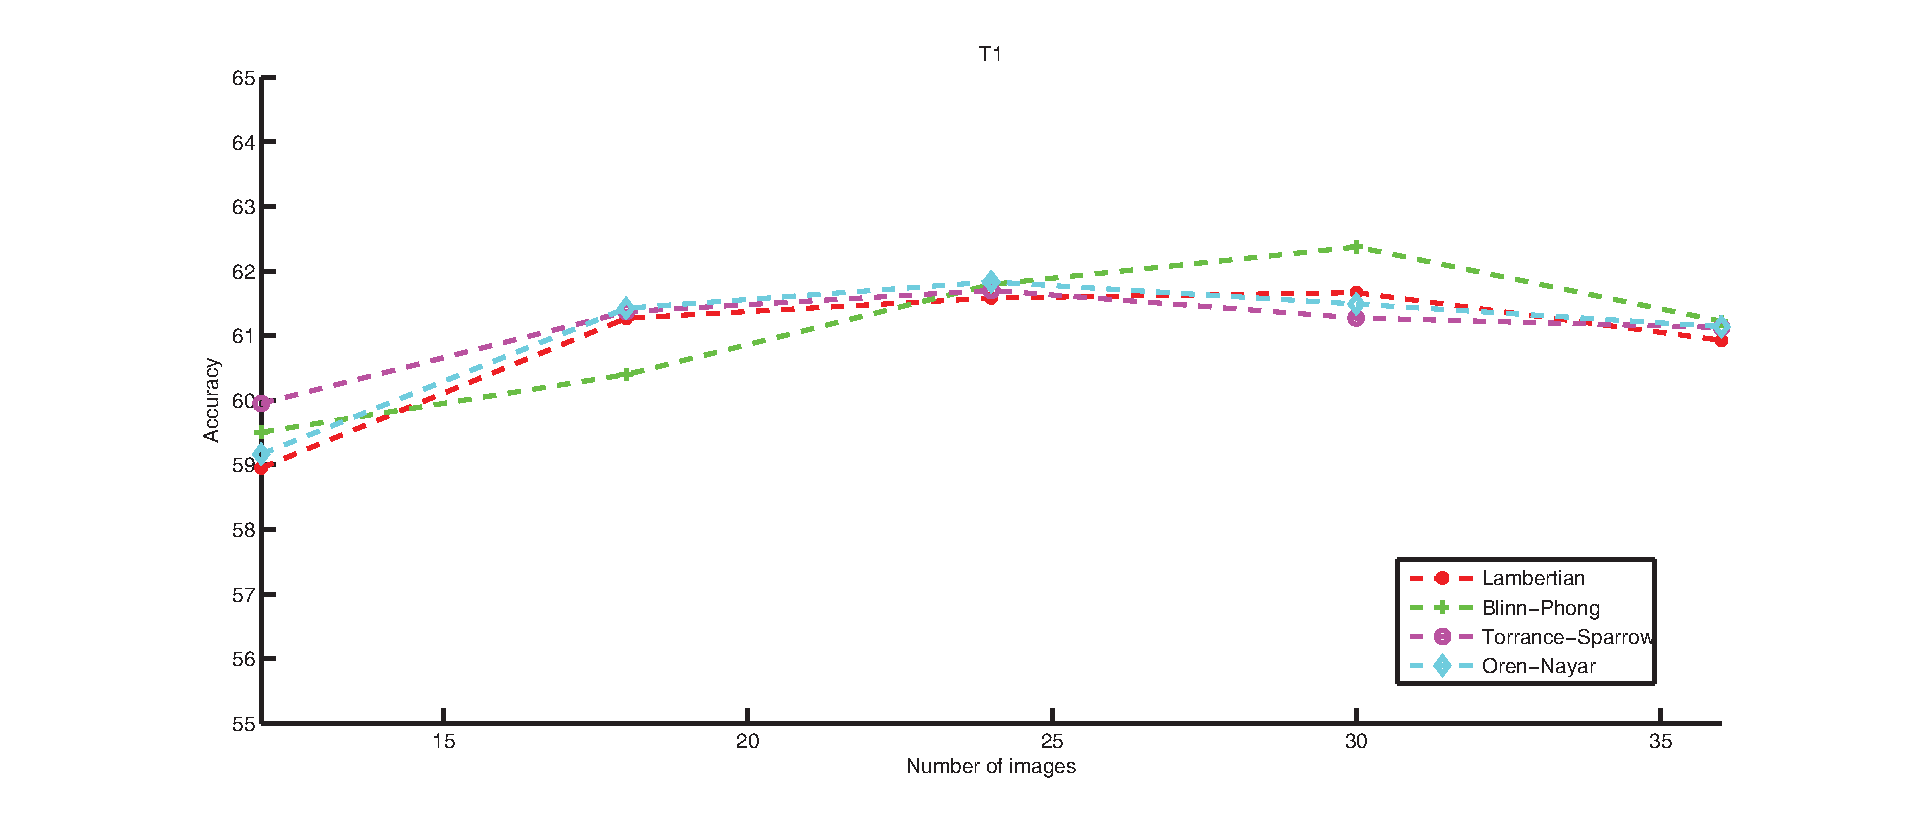
\epsfig{file=images/results/T1_specular.eps, width=0.75\linewidth}}
	\end{center}
	\caption{{\it Results on the T1 dataset for specular materials}}
	\label{fig:SpecularPlotB}
\end{figure}

